\documentclass{article}
\usepackage{CJKutf8}
\usepackage{multicol}
% Packages
\usepackage{lipsum} % For generating dummy text
\usepackage[top=1in, bottom=1in, left=1in, right=1in]{geometry}
\usepackage{hyperref}
\usepackage{pgfplots}
\usetikzlibrary{pgfplots.polar}
\usepackage{caption}
\captionsetup{font=small}
\usepackage{standalone}
\usepackage{listings}
\usepackage{xcolor} % For setting colors
\usepackage{amssymb}
\usepackage{amsmath}
\usepackage{algorithm}
\usepackage{algpseudocode}
\usepackage{afterpage}
\usepackage{placeins}
\usepackage{tikz}
\usepackage{enumitem}
\lstset{
  language=[LaTeX]TeX,
  breaklines=true,
  basicstyle=\ttfamily\small,
  keywordstyle=\color{blue},
  commentstyle=\color{green},
  backgroundcolor=\color{gray!10},
  frame=single,
  showspaces=false,
  showstringspaces=false,
}
\pgfplotsset{compat=1.17} % Use this to ensure compatibility with newer features
\setlength{\parskip}{6pt}
% Title and author
\title{Autonomous competence identification protocol: A dynamic ranking ladder system for blockchain applications}


\author{Tim Pechersky, Aivars Smirnovs}


\begin{document}
\begin{CJK}{UTF8}{gbsn}

    % \twocolumn
    \maketitle


    \begin{abstract}
        Meritocratic systems often struggle to identify and reward competence objectively. This paper proposes a novel protocol for establishing a dynamic ranking ladder system within trustless environments. By leveraging game-theoretic principles and dynamic systems theory, our protocol enables the autonomous identification of competence while mitigating potential sybil attacks. Participants engage in competitive "elections" within time-locked, tiered groups, with winners progressing to higher ranks. This process creates a quantifiable and verifiable measure of competence, represented by a tokenized rating. The protocol's time-based and cost-based mechanisms ensure that achieving high ranks requires genuine effort and skill, making it resistant to manipulation.  Potential applications include merit based blockchain consensus, decentralized social networks, DAO governance.
    \end{abstract}

    \section{Introduction}

    Traditional meritocratic models often falter due to the inherent difficulty of objectively identifying and rewarding competence.\cite{Arrow2000} This challenge is amplified in decentralized systems, where trust is minimized and the potential for manipulation is high. Existing consensus mechanisms, such as Proof-of-Work and Proof-of-Stake, may only proof that participant has either computational or financial power, but not necessarily competence needed, for example, to govern the protocol development. This hinders ability of decentralized systems developers to create robust governance and funding mechanisms that would be not pure power based, but also competence based.\cite{Rainer2023}\cite{Robin22} Ultimately leading researchers questioning viability of decentralized organizations as a concept.\cite{Xuan2024}

    This paper introduces a novel protocol designed to address this gap by establishing a dynamic ranking ladder system. Our protocol incentivizes participants to demonstrate their abilities through competitive "elections" within tiered groups. By requiring both time and financial commitment, we create a system that is resistant to Sybil attacks and fosters genuine competence development. This approach can be applied to various decentralized systems, including blockchain consensus mechanisms, where it can contribute to more robust and equitable governance.

    This research aims to:

    \begin{itemize}[nosep]
        \item Propose a methodology for creating a dynamic ranking system in a trustless environment.
        \item Analyze potential attack vectors and present robust resistance mechanisms.
        \item Discuss potential applications and benefits of the competence framework.
    \end{itemize}

    It is important to note that the proposed protocol is a theoretical construct that relies on having already established consensus mechanism to facilitate the protocol operation. Such could be executed on top of existing blockchain consensus mechanisms.

    \section{Protocol description}

    Protocol is based on breaking participants in to smaller groups with singular purpose of electing a winner. This process of election can be implemented as any sub-protocol that can take form of block building challenge, community discussion or more generally data exchange between participants and is not discussed in this paper. The only importance is that it must take multiple participants that must agree on leader, and that leader must be able to be verified by all participants.

    In order to make such groups interoperable based on same trust assumptions, yet free to define their own participation parameters, we introduce two distinct principal constant values constituting our protocol: (1) principal time constant $P_t$ and (2) principal asset cost $P_c$. These serve to create a common price and time relationship between any group to each other. We also add boundary case limitation $N_{min}$ - minimum number of participants required to form a group.

    Beside protocol wide constants, we allow Every group to have own properties:
    \begin{itemize}[nosep]
        \item id - a protocol wide unique group identifier
        \item $N$ - number of participants
        \item $T$ - minimum time, agreed by members, that's needed to finalize election
        \item $R$ - rank
        \item $S$ -  state - can be one of following:
              \begin{itemize}[nosep]
                  \item \textbf{created} - group is created and waiting for participants to join
                  \item \textbf{started} - group is started $ts_i$ time of start is recorded
                  \item \textbf{finalized} - group is finalized
              \end{itemize}
              % \item $X$ - stake requirement
    \end{itemize}


    Beyond that, for every participant there are two global properties:
    \begin{itemize}[nosep]
        \item  $P_r$ - rank of participant
        \item $P_g$ - group id last joined by participant
    \end{itemize}

    Participants can change groups only as long as their current and target group are not in "started" state. Whenever a group is started, it is expected to have at least $N_{min}$ participants and it must cause irreversible stake of participation $X_i$ to all participants balance:
    \begin{equation}
        \label{eq:group-fee}
        X_{id} = f(T_{id}) = \dfrac{P_t \cdot  P_c }{T_{id}}
    \end{equation}

    these costs further can be broken down in to equal stake subtracted from each participant account whenever group changes it's state to "started":
    \begin{equation}
        \label{eq:join-fee}
        stake = \dfrac{X_{id}}{ N_{id}}
    \end{equation}
    \documentclass{article} % Use an appropriate document class for your main document
\usepackage{tikz}
\usetikzlibrary{positioning, shapes.geometric}

\begin{document}

\begin{figure}[ht]
    \centering
    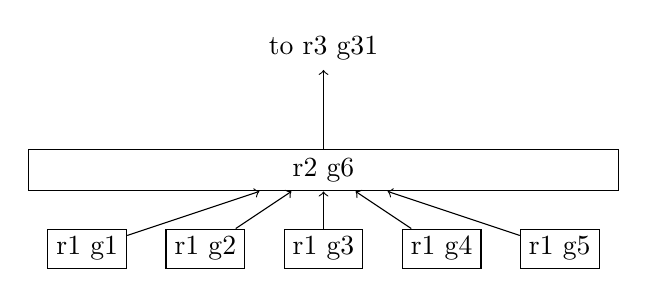
\begin{tikzpicture}[node distance=1cm and 1cm]
        % Bottom level blocks (5 participants)
        \foreach \x in {1,...,5} {
            \node[draw, rectangle, minimum width=1cm, minimum height=0.5cm] (P-\x) at (\x*1.5, 0) {};
            % Add "Rank X" text inside each block
            \node at (\x*1.5, 0) {r1 g\x};
        }

        % Single block for the game
        \node[draw, rectangle, minimum width=7.5cm, minimum height=0.5cm] (Game) at (4.5, 1) {r2 g6};

        % Connect participants to the game
        \foreach \x in {1,...,5}
            \draw[->] (P-\x) -- (Game);

        % Arrow pointing upwards from the top block with text "to r3"
        \draw[->] (Game.north) -- ++(0,1) node[above] {to r3 g31};
    \end{tikzpicture}
    \caption{Diagram illustrating the rank ladder. With minimum participant requirements of 5, 30 games are required to create a rank 3 game. Strong candidate would need only 2 wins to reach it.}
    \label{fig:game-connection}
\end{figure}


\end{document}
    the group can be finalized only after $T_{i}$ has elapsed since group start state transition. Then a winner can be declared and his rank $P_r$ in the state trie incremented to $P_r=P_r+1$ only if group rank $R$ is equal to $P_r$ before finalization. This process can be repeated and is illustrated on Fig. \ref*{fig:game-connection}.

    The staked assets further distributed in such manner that would avoid creation of positive feedback loop between groups and participants. Example of such would be nullifying these assets, therefore considering that $R+1$ state transition has intrinsic cost of $X_{id}$.


    \paragraph{Dynamic Proof-of-Authority.} As one can notice, the transfer of state is unidirectional from assets in to rank, and is time dependant, every transition can be seen as differential equation cost:
    \begin{equation}
        \label{eq:time-weighted-proof-of-authority}
        \$P_r = \$(P_r-1) + X_{id}
    \end{equation}
    while the rate of obtaining any rank $P_r$ itself is a unit step function dependent on time $t$:
    \begin{equation}
        \label{eq:time-weighted-proof-of-authority-1}
        P_r(t) = \lfloor \dfrac{t \cdot P_t \cdot P_c}{T_{min}} \rfloor
    \end{equation}

    \paragraph*{Frequency domain.}Observation in Eq.\ref{eq:time-weighted-proof-of-authority-1} highlights the dynamic nature of the protocol. Since it is showing linear-time invariant property, the dynamic systems theory\cite{Lynn86} may be applied to the protocol to analyze its stability and predict its future behavior.

    For example, $1/T_{min}$ represents frequency, hence analysis can be applied to understand phase and frequency relationship between groups with all power and system may be analyzed in s-domain used Laplace transforms. Variety of participants using different ${T_{min}}$ would result a dynamic competence ladder that can produce specific quorums at specific time points.



    \section{Sybil attack resistance}
    Ultimate outcome of protocol is representation of competence of an agent by storing his $R$ rank in the state trie. In order to ensure that such representation is not subject to manipulation, we must analyze security concerns.

    From a game theoretic perspective, adversary can be a group that produces a winner with $R$ rank that is higher than any other group in the system. However payment requirement defined in Eq. \ref{eq:group-fee} will be proportional to the number of participants in the group, contrary to the stake requirement fair participant is expected to pay (Eq. \ref{eq:join-fee}).

    While principal components defining fees allows ensure that any winner produced by any group is time and asset effort normalized.
    For example, in case of $T_{min} = P_t$, then equation \ref{eq:group-fee} reduces to:
    \begin{equation}
        \label{eq:join-fee-2}
        X_i = P_c
    \end{equation}

    If state transition of one participant's rank $R$ requires a commitment from $N_{min}$ participants, such as a participation fee $X_i$, we can demonstrate that the proposed ranking ladder introduces a non-linear compounding friction for potential malicious actors attempting to manipulate the system.

    For such an adversary the particular strategy depends strongly on the particular application of how the agents actually decide on the winner. If such a process is deterministic, the expected cost is simply
    \begin{equation}\
        \label{eq:direct-sybil-cost}
        X_g \cdot N_{min}^R
    \end{equation}. If an adversary is able to mix in with fair agents who are not sybils, and the process is not fully deterministic, then we can use the mathematical expectation for costs achieving specific rank via sybil attack described as
    \begin{equation}
        \mathbb{E}[\$R] = X_g \cdot \mathbb{E}[N_{\text{sybils}}(R)]
    \end{equation}

    Where $N_{sybils}(R)$ is a number of sybil accounts required to take quorum in a group, and hence obtain rank $R$.

    \paragraph{Actor likeleness and group fragmentation.}
    From Eq. \ref{eq:direct-sybil-cost} it can be seen that higher groups generally will be more expensive to manipulate, however in practice breaking groups in smaller may be desired to prevent overcomplexity of needed communication. This would imply that due to group fragmentation, an attacker mixing sybil accounts with fair players must strategically allocate accounts across groups for cost efficiency.

    Ability for participants to reason about the likelihood of a specific group to be a sybil attack is important in that context. If it seems like a group is likely to be a sybil attack, participants must be able to choose to not join the group. This can be done by reviewing the past state history of participants, groups he is joining and social graph arising from how votes are being allocated and can be done with dynamic systems methodology proposed in the end of previous section.

    While providing this level of visibility for participants to reason about may seem challenging, protocols like Continuous Voting Proposing Protocol (CVPP) \cite{cvpp} offer a clear definitions for system that will be transparent and easy to reason about, while in general, an automated system can be used to analyze the state trie and provide a clear view of the system.

    Additionally, we can use verification mechanisms, such as proof of location \cite{sheng2024bftpolocbyzantinefortifiedtrigonometric} or proof of personhood \cite{WorldCoin2024} or from use of quadratic voting systems which already shown to be helpful in blockchain governance field \cite{Buterin20}\cite{Benhaim2024}.

    If all results are visible and easy to reason about, then, from outset, this means that for any protocol participant, confidence over group conducting a sybil attack will increase as $R$ of group increase, hence they will be more likely to refuse joining group with such, resulting a sybil attack cost close to Eq. \ref{eq:direct-sybil-cost}:
    \begin{equation}
        \lim_{R \to \infty} \mathbb{E}[N_{\text{sybils}}(R)] = N_{\text{min}}
        \label{eq:limit-nmin}
    \end{equation} Where $N_{min}$ is amount of peers required to join the group. Hence, Eq. \ref{eq:direct-sybil-cost} can be used to estimate cost of sybil attack. At the same time, for the agent who is relying on his pure competence and wins each group fairly, by being able to align agents to vote for him, same cost would be only \begin{equation}
        \$R = stake*R
    \end{equation}
    Hence, the agent competence can be put at stake when making a any arbitrary decision that uses $R$ as stake. This may take form of taking privileged action with optimistic approval and so on, only condition required to keep agent game-theoretically fair is that action impact must be lower than the cost of obtaining rank.
    \begin{equation}
        \$TVL <<  X_g \cdot N_{min}^R
    \end{equation}

    Total value locked must be substantially lower then a cost for obtaining rank due to reason that empirical studies are needed to see how fast will required sybil count converge (Eq. \ref{eq:limit-nmin}) in practice with a different voting systems. This strongly depends on how much stochastic and transparent is such a process.


    \subsection{Quorum Resonances}
    \label{sec:time-constraint}

    As discussed in the previous section, any overt sybil attack requires multiple groups to be held in order to establish a sufficient ranking within the system.

    Therefore, the intrinsic value of a tokenized competence rating is determined not only by financial effort and success among peers but also by the time invested in continuously improving one's position within the system. Even with parallel attack instances, an attacker would still require $t_{attack}(R) = t_c \cdot R$ time to reach rank $R$. This extended duration allows protocol members ample opportunity to detect and respond to the attack.
    Moreover, the Eq. \ref{eq:time-weighted-proof-of-authority-1} shows that system can be analyzed in time and frequency domains, hence it is possible to analyze sybil attacks not just as a function of time, but also as a function of phase, use complex frequency domain analysis etc.

    Also given the initial goal to facilitate protocol for a subjective reasoning matters, it is arguable what it even is - an "sybil attack" or just a "different opinion". Assuming there exist different opinions, and using the proposed s-domain methodology, competing opinion groups have a way of creating a quorum resonance, where the opinion direction itself can oscillate. All it takes it to have same $T_{min}$ for competing groups that begin their election process at phase difference of $\pi$. This can be visualized in following plot \Ref{fig:processes}.:

    \begin{figure}[ht]
        \centering
        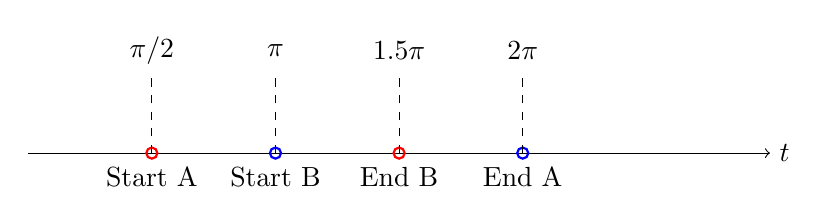
\begin{tikzpicture}
            % Define the x-axis
            \draw[->] (0,0) -- (3*3.14,0) node[right] {$t$};

            % Define the first process (point at Pi)
            \draw[blue, thick] (3.14,0) circle (2pt);
            \draw[blue, thick] (3.14*2,0) circle (2pt);
            \node[] at (3.14*0.5,1.3) {$\pi/2$};
            \node[] at (3.14,1.3) {$\pi$};
            \node[] at (3.14*1.5,1.3) {$1.5\pi$};
            \node[] at (3.14*2,1.3) {$2\pi$};

            % Define the second process (point at Pi/2)
            \draw[red, thick] (1.57,0) circle (2pt);
            \draw[red, thick] (1.57+3.14,0) circle (2pt);

            % Add labels for the timing diagram
            \node at (1.57,-0.3) {Start A};
            \node at (3.14,-0.3) {Start B};
            \node at (3.14*2,-0.3) {End A};
            \node at (1.57+3.14,-0.3) {End B};

            % Add dashed lines to indicate the timing
            \draw[dashed] (1.57,0) -- (1.57,1);
            \draw[dashed] (3.14,0) -- (3.14,1);
            \draw[dashed] (3.14*2,0) -- (3.14*2,1);
            \draw[dashed] (1.57+3.14,0) -- (1.57+3.14,1);
        \end{tikzpicture}
        \caption{Timing diagram showing two opposite opinion groups finalizing their election process at different time points. The groups have the same $T_{min}$ but with a phase difference of $\pi$.}
        \label{fig:processes}
    \end{figure}

    Further, more complicated systems can be imagined, if such groups are many and they allocate their power to reason in alliance manner, creating local quorum resonances, that can be analyzed in frequency domain, and can be used to predict future behavior of the system \ref{fig:processes-sinusoidal}.

    \begin{figure}[ht]
        \centering
        \begin{tikzpicture}
            % Define the x-axis
            \draw[->] (0,0) -- (10,0) node[right] {$T_{min}$};

            % Define the y-axis
            \draw[->] (0,-2) -- (0,2) node[above] {Quorum power};

            % Define the first process (sine wave)
            \draw[domain=0:10,smooth,variable=\t,blue] plot ({\t},{sin(360*\t/10)});
            \node[blue] at (10,1) {Opinion 1};

            % Define the second process (sine wave shifted by half period)
            \draw[domain=0:10,smooth,variable=\t,red] plot ({\t},{sin(360*\t/10 + 180)});
            \node[red] at (10,-1) {Opinion 2};

            % Add labels for the half period shift
            \draw[dashed] (5,-2) -- (5,2);
            \node at (5,-2.5) {$\pi$};

            % Add labels for the full period
            \draw[dashed] (10,-2) -- (10,2);
            \node at (10,-2.5) {$2\pi$};

        \end{tikzpicture}
        \caption{Diagram showing two competing group sets over same subject having their groups $T_min$ same but with same phase difference of $\pi$. Sinusoidal waves are for illustrative purpose, in reality, the groups would have different $T_{min}$ and could be more complex
            \label{fig:processes-sinusoidal}}
    \end{figure}

    From this diagram we can see that two opposite opinions can take quorums in different time $t$.

    \section{Conclusion}

    This paper introduces a novel protocol for establishing a dynamic ranking ladder system in trustless environments. By leveraging game-theoretic principles and dynamic systems theory, our protocol enables the autonomous identification of competence while mitigating Sybil attacks. The time-based and cost-based mechanisms ensure that achieving high ranks requires genuine effort and skill and even completely opposite opinions have ability to co-exist.

    This protocol offers a promising foundation for building more robust and equitable decentralized governance systems. It has the potential to improve blockchain consensus mechanisms, enhance DAO decision-making, and foster healthier online communities.

    Further work is required to analyze the protocol's behavior and effectiveness using dynamic system theory and to explore its integration with existing decentralized platforms.






    \clearpage

    % \appendix
    % \section{Appendix A: Listings}
    % 
\begin{algorithm}
\caption{Basic Autonomous competence identification}
\begin{algorithmic}[1] % Enables line numbering
\State \textbf{Prerequisites:} Minimal group size $N_{min}$, Time constant $t_{c}$, Participation cost $X_g$, Competence Asset $C_i$, Protocol Treasury $T$, Minimal turn count ${M, M > 2}$
\State \textbf{Process:}
\Procedure{Preparation}{}
    \State Instance is created at timestamp $t_0=t$, with creators personal join requirements $X_a$
    \State Participants join the group and lock in a commitment: $N_{min} \times (X_g+X_a) \rightarrow T$
    \State Joining period ends at $t_1  \ge t_c + t_0$
\EndProcedure
\Procedure{FirstTurn}{}
    \While{$t_1 + t_c \ge t$}
        \If{new Proposal}
        \State Record ${P_i}$
        \State Record $i$
        \EndIf
    \EndWhile
    \If{Group is full or joining timeout}
        \State Members exchange encrypted proposals (MPC).
    \EndIf
\EndProcedure
\Procedure{DecryptProposals}{}
    \If{Timeout or all proposals received}
        \State Members decrypt proposals using threshold encryption.
    \EndIf
\EndProcedure
\Procedure{RegularTurn}{}
    \State Submit new encrypted proposals.
    \State Submit encrypted votes and zk-proof of valid vote.
\EndProcedure
\Procedure{CalculateRoundScores}{}
    \If{Round ends or all votes \& proposals submitted}
        \State Use TSS cryptography to decrypt everything.
        \State Calculate round scores.
    \EndIf
\EndProcedure
\Procedure{RepeatUntilXProposals}{}
    \State Repeat steps 3-5 until a total of X proposals.
\EndProcedure
\Procedure{FinalizeRankings}{}
    \State Count total votes and sort proposals.
\EndProcedure
\end{algorithmic}
\end{algorithm}


    % \clearpage
    \bibliographystyle{ieeetr}
    \bibliography{../references.bib}

    \clearpage\end{CJK}
\end{document}
